\documentclass[onecolumn, 11pt, draftclsnofoot]{IEEEtran}

\usepackage{epsfig,graphics,epsf,amsfonts,color,mathrsfs,amssymb,bm,caption,algorithm,algorithmic}
\usepackage{url}

\usepackage{amsmath}
\newcommand{\bsb}{\boldsymbol}
\newcommand{\mb}{\mathbf}
\newcommand{\mc}{\mathcal}
\newcommand{\mexpc}{\mathrm{E}}
\newcommand{\ve}{\mathrm{vec}}
\newcommand{\toep}{\mathcal{T}}
\newcommand{\tr}{\mathrm{tr}}
\newcommand{\tred}{\color{red}}
\textheight=9.2in
\DeclareCaptionLabelFormat{lc}{\MakeLowercase{#1}~#2}
\captionsetup{labelfont=sc,labelformat=lc}
\renewcommand{\figurename}{Figure}
\renewcommand{\theequation}{R\arabic{equation}}
\usepackage[numbers]{natbib}

\setcounter{equation}{14}
\setcounter{figure}{1}
\setcounter{table}{1}


%\hyphenation{op-tical net-works semi-conduc-tor}
\begin{document}
The authors once again appreciate the helpful comments from the editor and both
reviewers.
Throughout this response letter, we will follow the following notational
rules for citations and references:
\begin{itemize}
  \item Citations: references in this response letter are cited with prefix
  ``R'' (e.g. [R 1]) whereas references in the original manuscript are cited
  without prefix (e.g. [1]).
  \item Equations: equations in this response letter are referred to as
  ``Eq.~(R1)''  while those in the original manuscript as ``Eq.~(1)''.
  \item Figures: figures in this response letter are referred to as
  ``FIGURE~1''  while those in the original manuscript as ``Fig.~1''.
\end{itemize}
Also the reference numbers for equations, figures and tables
consistently continue to count up from their counterparts in our previous
response letter.

\begin{center}
  {\LARGE \textbf{Authors' Response to Reviewer 1}}
\end{center}

% ~\citep[R][]{cheng2013thermal}
% \begin{align}
%   sfsdf
%   \label{eq:test}
% \end{align}
% \eqref{eq:test}
% \begin{figure}[!t]
%   \centering
%   \includegraphics[width=0.75\columnwidth]{./figs/test.eps}
%   \caption{Average throughput.}
%   \label{fig:test}
% \end{figure}
% Fig.~\ref{fig:test}

 
%%%%%%%%%%%%%%%%%%%%%%%%%%%%%%%%%%%%%%%%%%%%%%%%%%%%%%%%%%%%%%%%
\noindent
\emph{1. \ldots However, the method (Section III.B) has still some points to be
clarify. The main concern is why the authors transform the original problem (11)
into a more complex problem (13). The assignment variables x play a key role
here, but the authors do not explain what they are modeling with the second and
third component of x; also, in the expression of x, the meaning of indexes i and
j is not revealed.}

\noindent \textbf{Authors' response:} 
Thank you for the comment. As we have stated in our response to comment 5 in our
previous response letter as well as the revised manuscript, there is a
one-to-one mapping between the 3-D permutation matrix
$\mathbf{x}^{(m)}\in\mathcal{S}$ (Eq.~(12)) and the vector mapping function
$\bm{\psi}^{(m)}[p] = [\psi_1^{(m)}[p], \psi_2^{(m)}[p]]$. In other words, the
original problem (11) and problem (13) are equivalent and neither one is more
complex than the other. Rewritting our design objective (11) into (13) simply
aims to reduce the MoDiv design problem into a Q3AP in its most typical form.

By second and third component of $x$ we presume that the reviewers meant the
second and third dimension of the 3-D permutation matrix $\mathbf{x}^{(m)}$. As
$x_{pij}^{(m)}=1$ if $\psi_1^{(m)}[p] = \psi_0[i]$ and $\psi_2^{(m)}[p] =
\psi_0[j]$ and otherwise $x_{pij}^{(m)}=0$, the second dimension of
$\mathbf{x}^{(m)}$ (indexed by $i$) defines the modulation mapping function $\psi_1[\cdot]$ at the
first transmitter with respect to the reference mapping function
$\psi_0[\cdot]$ (Gray mapping), and the third dimension of $\mathbf{x}^{(m)}$
(indexed by $j$) defines the modulation mapping function $\psi_2[\cdot]$ at the second
transmitter. Consequently, $\mathbf{x}^{(m)}$ as a whole defines the 2-D vector
mapping function $\bm{\psi}^{(m)}[\cdot]$ with respect to Gray mapping
$\psi_0[\cdot]$. $i,j=0,\ldots,Q-1$ are simply indexing variables similar
to $p$ whose meanings are implicitly defined with $\mathbf{x}^{(m)}$.
$x_{pij}^{(m)}=1$ means that during the $m$-th retransmission, the first transmitter maps label $p$ to the same constellation
symbols as Gray mapping maps label $i$ to, and the second transmitter maps label
$p$ to the same constellation symbols as Gray mapping maps label $j$ to.

Here we demonstrate a 3-D permutation matrix $\mathbf{x}^{(m)}$ and the
equivalent $\bm{\psi}^{(m)}[\cdot]$ for QPSK ($Q=4$) in FIGURE~\ref{fig:mapping}
and TABLE~\ref{table:x}.


\begin{table}[!t]
  \renewcommand{\arraystretch}{1.3}
  \caption{The indices $(p,i,j)$ where $x_{pij}^{(m)}=1.$}
  \label{table:x}
  \centering
  \begin{tabular}{c|c|c}
    \hline
    $p$ & $i$ & $j$  \\
    \hline
    0 &  0 & 0 \\
    1 & 3 & 3 \\
    2 & 2 & 1 \\
    3 & 1 & 2 \\
    \hline
  \end{tabular}
\end{table}

\begin{figure}[h]
  \begin{minipage}[b]{0.32\linewidth}
    \centering
    \centerline{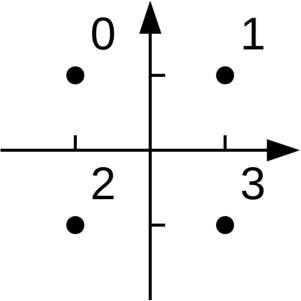
\includegraphics[width=3.0cm]{./figs/gray.pdf}}
    \centerline{(a) $\psi_0[p]$ (Gray mapping)}
    \medskip
  \end{minipage}
  \hfill
  \begin{minipage}[b]{.32\linewidth}
    \centering
    \centerline{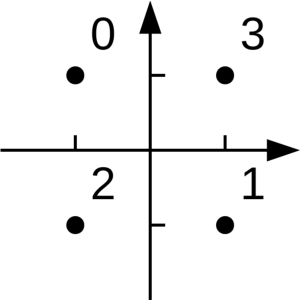
\includegraphics[width=3.0cm]{./figs/tx1.pdf}}
    \centerline{(b) $\psi_1^{(m)}[p]$}
    \medskip
  \end{minipage}
  \hfill
  \begin{minipage}[b]{.32\linewidth}
    \centering
    \centerline{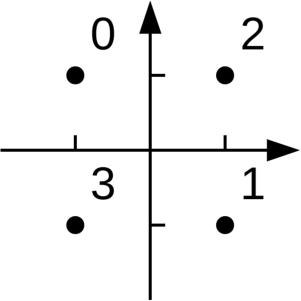
\includegraphics[width=3.0cm]{./figs/tx2.pdf}}
    \centerline{(c) $\psi_2^{(m)}[p]$}
    \medskip
  \end{minipage}
  \caption{Constellation mapping for the Gray mapping. Label $p$
  are marked next to each constellation symbol.}
  \label{fig:mapping}
\end{figure}

As you can see, $\mathbf{x}^{(m)}$ are already well defined by stating that
it is a permutation matrix satisfying Eq.~(12). To make the one-to-one
relationship between $\mathbf{x}^{(m)}$ and $\bm{\psi}^{(m)}$ more clear, we
changed back to our original notation, i.e. $x_{pij}^{(m)}
= 1$ if $ \bm{\psi}^{(m)}[p] = [\psi_0[i], \psi_0[j]]^T$ and otherwise $x_{pij}^{(m)} =
0$ in the first paragraph of Sec. III B. Also in order to clarify the meaning of
the second and third dimension of $\mathbf{x}^{(m)}$, in the revised manuscript
we explicitly state that $\psi_1^{(m)}$ and $\psi_2^{(m)}$ are defined by the
1st, 2nd and 1st, 3rd dimension of $\mathbf{x}^{(m)}$, respectively.

\vspace{0.5cm}

%%%%%%%%%%%%%%%%%%%%%%%%%%%%%%%%%%%%%%%%%%%%%%%%%%%%%%%%%%%%%%%%
\noindent
\emph{2. the original formulation of x is more clear than using Kronecker delta.
}

\noindent \textbf{Authors' response:}
As explained in our response to comment 1, we have changed back to our original
formulation of $\mathbf{x}$ in the first paragraph of Sec. II.

\vspace{0.5cm}

%%%%%%%%%%%%%%%%%%%%%%%%%%%%%%%%%%%%%%%%%%%%%%%%%%%%%%%%%%%%%%%%%
\noindent
\emph{3. what do you mean with ``$\psi_0$ represents Gary mapping'' (page 2,
column 2, line 13)}

\noindent \textbf{Authors' response:}
By ``$\psi_0$ represents Gray mapping'' we meant, similar to the definition in
the first paragraph of Section II, that $\psi_0[p]$ is a one-on-one mapping
between $p=0,\ldots,Q-1$ to the constellation symbols in $\mathcal{C}$.
Specifically, Gray mapping, which has been widely used in digital
communication systems for QAM, QPSK modulation, etc., is demonstrated in FIGURE
1(a) in our previous response letter. It is also noted that Gray mapping
generally means that the labels corresponding to the closest pair of
constellation points differ by only one bit so as to minimize the BER. Also,
there is no unique definition of Gray mapping. For instance, for 16-QAM, two
types of Gray mapping are illustrated in Sec.7.1.3~\citep[R][]{TS36.211} and
Fig.2(a)~[5], respectively, and our MoDiv design procedure is applicable
regardless which specific mapping is used. In fact, $\psi_0$ can be any given
constellation mappings and it is just used as a ``reference mapping function''
in order to introduce the permutation representation $\mathbf{x}$.
The Gray mapping assumption is simply based on the fact that most CoRe schemes
uses Gray mapping for the original transmission.

To clarify the meaning of $\psi_0$, we have re-written it into a similar form as
$\psi_a^{(m)}$ as in the first paragraph of Sec. II in the hope that our readers
can see that $\psi_0$ is simply a specific mapping function as defined
previously.
Since the exact form of Gray mapping can be found at almost any classical
wireless communication
textbook~\citep[R][]{proakisdigital,molisch2007wireless,goldsmith2005wireless},
given the page limit, it is not necessary to include a more detailed
definition or a reference in our manuscript.



\vspace{0.5cm}

%%%%%%%%%%%%%%%%%%%%%%%%%%%%%%%%%%%%%%%%%%%%%%%%%%%%%%%%%%%%%%%%%%
\noindent
\emph{4. why $\lambda = 1/(4\sigma^2)$ in the proof of proposition 1?}

\noindent \textbf{Authors' response:}
Comparing Eq.(R8) with Eq.(6), we simply replace $\mathbf{v}$ with
$\mathbf{A}^{(n)}\mathbf{e}^{(n)}[p,q]$ and $\lambda = 1/(4\sigma^2)$. In order
to avoid a similar confusion from our readers, now this connection is explicitly
drawn in the proof of Proposition 1 in our manuscript.
 
\vspace{0.5cm}

%%%%%%%%%%%%%%%%%%%%%%%%%%%%%%%%%%%%%%%%%%%%%%%%%%%%%%%%%%%%%%%%

Once again, we greatly appreciate the reviewer's comments and suggestions
that helped to continuously improve our revised manuscript. 

\newpage
\begin{center}
{\LARGE \textbf{Authors' Response to Reviewer 2}}
\end{center}

%%%%%%%%%%%%%%%%%%%%%%%%%%%%%%%%%%%%%%%%%%%%%%%%%%%%%%%%%%%%%%%%%%%%%
\noindent
\emph{The application scenario investigated by the authors is timely and of
great interest. This reviewer appreciates the efforts the authors have devoted
to revise the paper and thinks it is worth to publish the proposed approach and
results based on it on IEEE communications letters.}

\noindent \textbf{Authors' response:}
Once again we would like to extend our gratitude and appreciation for the
reviewer's recommendation and for affirming the contribution of this work.

\vspace{0.5cm}

 %\newpage
\bibliographystyle{IEEEtranN}
\bibliography{IEEEabrv,refs.bib}
\end{document} 